\chapter{Grundlagen}
\label{sec:Grundlagen}
Die Leistungselektronik ist ein komplexes Thema das im Grunde mit dem Beginn der Elektrizität beginnt, die Wandlung und Übertragung von Strom stellte die ersten großen Hindernisse dar. Insbesondere die Entscheidung zwischen Wechsel- und Gleichspannung in den Übertragungs- und Verteilnetzen stellte eine erste Große Debatte dar. Durch die Weiterentwicklung in der Halbleitertechnik zeigt sich, dass Gleichstromtechnik insbesondere bei langen Übertragungsstrecken Vorteile gegenüber der verbreiteteren Wechselstromtechnik besitzt. Um die Anforderungen und Zusammenhänge verstehen zu können, werden Details zur Elektrolyse, zu Stromrichtern sowie Komponenten und der verwendeten Simulationsumgebung dargestellt.


\section{Wasserstoff-Elektrolyse}
\label{sec:Elektrolyse}
Unter Wasserstoff-Elektrolyse versteht man grundlegend die Funktion Wasser in seine Bestandteile Wasserstoff und Sauerstoff zu spalten. Die verbreitetste Variante ist die \gls{AEL}, welche bereits im großen Maßstab von bis zu zwei Giga Watt eingesetzt wird \cite{2GWely}. Des weiteren wird viel Potential in der Weiterentwicklung der \gls{PEM} Elektrolyse gesehen, da diese durch einen simpleren Aufbau und höhere Stromdichten bessere Skalierbarkeit bieten kann. Außerdem wird die \gls{HTEL} verwendet, wenn sich die Nutzung von Prozess technischer Abwärme anbietet, wodurch der Gesamtwirkungsgrad steigt \cite{Elektrolyse}.\\
Das Prinzip der \gls{AEL} wird, im Gegensatz zur neueren \gls{PEM}, Elektrolyse bereits seit langer Zeit verwendet und optimiert. Die \gls{AEL} benötigt in der Regel eine wässrige KOH-Lauge und kann durch Reihenschaltung der Zellen Wasserstoff und Sauerstoff mit erhöhtem Druck von Beispielsweise 30 Bar bereitstellen. Die Entwicklung und insbesondere Steigerung der Stromdichte und Effizienz brachte in den letzten Jahren jedoch keine großen Änderungen. Der Spannungswirkungsgrad liegt zwischen 62 und 82 Prozent \cite{NOWH2}.\\
Die \gls{PEM} Elektrolyse bietet Vorteile durch erhöhte Stromdichte, bei größeren Anlagen spart dies unter anderem Platzbedarf, außerdem ist zu erwarten, dass Druckelektrolyse bis 100 Bar möglich ist. Jedoch gibt es noch Optimierungsbedarf bei der  Langlebigkeit der Membranen und der benötigten Edelmetalle \cite{NOWH2}. \\
Die \gls{HTEL} nutzt die Vorteile durch höhere Temperatur, welche auf der Seite der Thermodynamik Vorteile für die Elektrische-Effizienz bringen, jedoch hohe Anforderungen an die verwendeten Materialien stellen. Daher ist die Festoxid Elektrolyse noch in einer Grundlagenforschung im Laborstadium. Da fast alle Festoxid-Zellen umkehrbare Eigenschaften besitzen ist das Interesse an ihnen besonders groß, dies ermöglicht die direkte Rückverstromung des Wasserstoffs. Jedoch wird hier ebenfalls noch eine Materialoptimierung sowie Verbesserung der Langzeiteigenschaften benötigt.\\

\begin{figure}
	\centering
	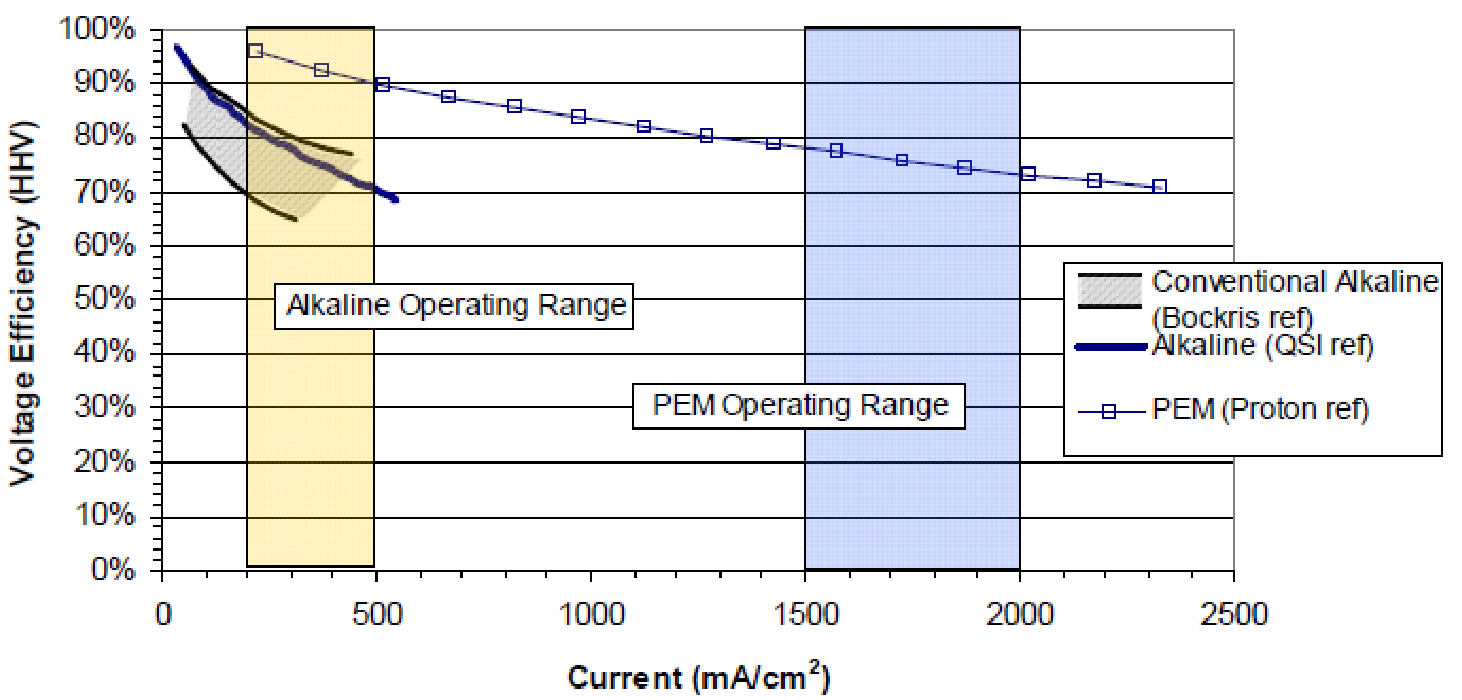
\includegraphics[width=0.7\linewidth]{content/Grafiken/Ely-Efficiency}
	\caption[Elektrolyseur Spannungseffizienz]{Elektrolyseur Spannungseffizienz \cite{NOWH2}}
	\label{fig:ely-efficiency}
\end{figure}


\section{Stromrichter}
\label{sec:Stromrichter}
Allgemein kann man jede Schaltung die zur Strom- und Spannungsversorgung dient als Stromrichter bezeichnen, dabei wird unterschieden zwischen Wechsel- und Gleichspannungsvarianten. Außerdem kann bei Netzanwendungen in gesteuerte, Netz-gesteuerte und ungesteuerte unterschieden werden, sowie die Umsetzung einer \gls{PFC} betrachtet werden. 
		\subsection{Gleichrichter}
		Ein Gleichrichter wird verwendet, um aus einer Wechselspannung eine Gleichspannung zu erzeugen. Die einfachste Form ist der Diodengleichrichter, dieser kann für einphasige Wechselspannung durch eine einzelne Diode realisiert werden. Jedoch würde so nur die halbe Periode des Sinus am Ausgang zur Verfügung stehen, da die Diode nur während der positiven Halbwelle Leitet. Dies lässt sich durch die Ergänzung zum Brückengleichrichter mit vier und für dreiphasige Anwendungen mit sechs Dioden ausgestattet ist.\\
		Anhand des Diodengleichrichters wird schnell klar, dass eine solche Schaltung nur bedingt für einen gewünschten Stromverlauf sorgt. In Abbildung \ref{fig:B6DiodRect} sind Netzspannung und Strom dargestellt, der Stromverlauf zeigt Starke Sprünge und der gewünschte Sinusförmige Verlauf ist nur schwer erkennbar. Außerdem lässt sich mit dieser Schaltung die Ausgangsspannung sowie der Strom nicht variieren.
		\begin{figure}[H]
			\centering
			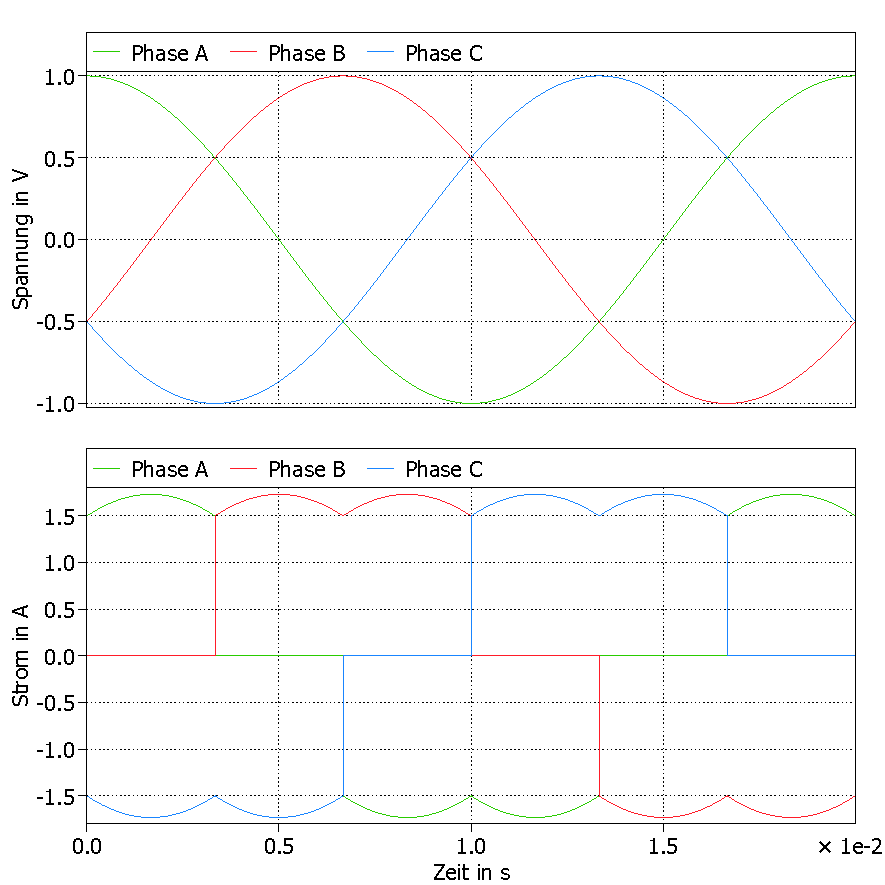
\includegraphics[width=0.7\linewidth]{content/Grafiken/B6-Diodengleichrichter-Eingangsverlauf}
			\caption{Strom und Spannungsverlauf am B6 Diodengleichrichter}
			\label{fig:B6DiodRect}
		\end{figure}
		
		Für Elektrolyseanlagen mit mehreren Megawatt Leistung müssen Zwangsweise Leistungshalbleiter parallelisiert werden, da bei Spannungen bis 1000 V die Ströme für einzelne Halbleiter zu hoch sind. Außerdem bietet die Parallelisierung durch Interleaving und Phasenverschiebung deutliche Vorteile für die Verzerrung und damit Filterung. Durch Thyristor basierte Schaltungen können große Leistungen effizient umgesetzt werden, jedoch führen diese zu deutlichen Verzerrungen des Stromverlaufs und schlechterem Leistungsfaktor. Daher benötigen diese passive oder aktive Filter, welche die Systemkosten erhöhen \cite{HydrogenElectronicTopologies}.
		Als Alternative dazu werden \gls{AFE} Gleichrichter eingesetzt diese bieten deutlich geringere Verzerrungen und völlige Freiheit bei der Regelung des Eingangsstroms. Daher können die Filter und Blindleistungskompensation in diesem Fall eingespart werden \cite{HydrogenElectronicTopologies}.
		
		\subsection{DC-DC Wandler} \label{sec:Buck}
		Der Hoch- und Tiefsetzsteller sind essenzielle Topologien und bestehen im wesentlichen aus zwei Halbleitern und einer Induktivität. In Abb. \ref{fig:buck} ist die Schaltung für einen Tiefsetzsteller zu sehen. Über das \gls{D} des Schalters kann die \gls{Ua} eingestellt werden, dabei sind die Parameter \gls{Ue}, Lastimpedanz sowie Wert der Induktivität relevant. Die Ausgangsspannung lässt sich im nicht lückendem Betrieb über den Zusammenhang $U_{out}=D\cdot U_{in} $ berechnen \cite{schmidtwalter}.\\
		\begin{figure}
			\centering
			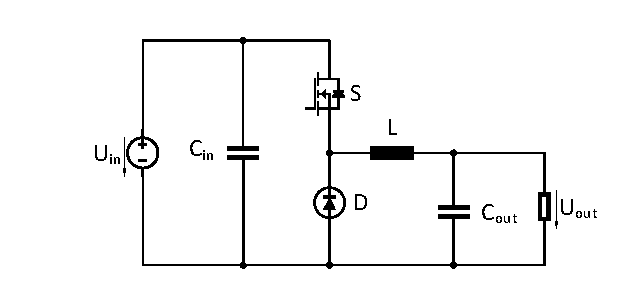
\includegraphics[width=0.7\linewidth]{content/Grafiken/Buck}
			\caption[Tiefsetzsteller]{Tiefsetzsteller}
			\label{fig:buck}
		\end{figure}
		Die Speicherdrossel des Tiefsetzstellers kann über Formel \ref{eq:BuckL} ausgelegt werden, der gewünschte Stromrippel wird dazu beispielhaft auf maximal 30 Prozent des \gls{Ia} festgelegt \cite{schmidtwalter}.
		\begin{equation}
			\label{eq:BuckL}
			L=\dfrac{U_{emax}-U_{a}}{f\cdot 0,3 \cdot I_{a}}\cdot \dfrac{U_{a}}{U_{emax}}
		\end{equation}
		Wenn die Eingangsspannung durch einen, wie in Abb. \ref{fig:B6DiodRect} dargestellten, Dreiphasigen Diodengleichrichter implementiert ist, kann die Eingangsspannung mit $U_{LL} \cdot \sqrt{2}$ berechnet werden. Daraus folgt Formel \ref{eq:BuckLB6} bezogen auf die Phasenspannungen. \\
		\begin{equation}
			\label{eq:BuckLB6}
			L=\dfrac{U_{LL} \cdot \sqrt{2}-U_{a}}{f\cdot 0,3 \cdot I_{a}}\cdot \dfrac{U_{a}}{U_{LL} \cdot \sqrt{2}}
		\end{equation}
		Eine weitere Optimierungsmöglichkeit bietet das Interleaving, hierbei werden zwei Schaltungen parallel betrieben und die Regelung gekoppelt, dass Sie abwechselnd schalten. Dies ermöglicht es zum einen die Drosseln besser auslasten zu können und zum anderen den Rippel zu halbieren. 
		
		
		\subsection{Power Factor Correction (PFC)}
			Die \gls{PFC} ist eine nötige Maßnahme um den Blindleistungsanteil im Netz zu reduzieren und wird daher in aktuellen Geräten Standardmäßig implementiert. Ein Beispiel aus der Industrie bei dem bereits eine einfache Blindleistungskompensation durchgeführt wurde, war bei Leuchtmitteln mit Halogenröhren. Diese wurden zur Erzeugung der nötigen Spannung mit einem Transformator ausgestattet, welcher jedoch Blindleistung verursachte, dies konnte durch einfache Ergänzung eines Kondensators optimiert werden. \\
			In gängigen Gleichrichtersystemen werden getrennte Einheiten bestehend aus einer dreiphasigen PFC-Gleichrichterschaltung und einem Gleichspannungswandler (DC/DC-Buck-Wandler) eingesetzt, um die Anforderungen zu erfüllen. Die Regelung der beiden Wandlerstufen ist in der Regel entkoppelt, wobei der Gleichrichter sinusförmige Netzströme zieht und der nachfolgende DC/DC-Wandler die Spannung auf den erforderlichen Ausgang anpasst. Auf der Suche nach kompakten und leichten Systemen sind hohe Schaltfrequenzen notwendig, was jedoch zu erhöhten Schaltverlusten und verringerter Wandlereffizienz führen kann. Um dies zu adressieren, werden fortgeschrittene Modulationstechniken wie Einfügen der dritten harmonischen und Raumzeigermodulation möglich. Alternativ kann auch Diskontinuierliche Pulsweitenmodulation (DPWM) als Methode zur Reduzierung der Schaltverluste in dreiphasigen PFC-Gleichrichtern verwendet werden, um sinusförmige Eingangsströme und eine konstante Gleichspannung sicherzustellen. Im Gegensatz dazu müssen Einstufen-Wandlersysteme beide Anforderungen gleichzeitig erfüllen, während Zweistufen-Systeme trotz niederfrequenter Spannungsschwankungen im Zwischengleichspannungsnetz eine konstante Ausgangsspannung sicherstellen können.			
			
\section{IAF Rectifier }
Der \gls{IAF} Gleichrichter wurde erstmals vorgestellt in \cite{IAFfirst} im Jahr 1997, zur Verwendung in Photovoltaik Anwendungen. Dieser besteht für den Hauptleistungspfad aus einem Diodengleichrichter. Um sinusförmige Ströme in allen drei Phasen einzuprägen wird dieser durch ein Netzwerk aus bidirektional Sperrenden Leistungshalbleitern mit einer Induktivität und Halbbrücke ergänzt, dies wird als \gls{THI} Schaltung bezeichnet. Durch die Integration des Filters in den Leistungspfad, wird keine externe Blindleistungskompensation benötigt und die Filter können kleiner ausfallen. Aufgrund des ungesteuerten Diodengleichrichters wird jedoch eine anschließende Spannungsregelung durch einen Tiefsetzsteller benötigt \cite{ThesisSchrittwieserBuckTypePFC_2017}.\\
Das Netzwerk aus bidirektionalen Schaltern, auch als \gls{IVS} bezeichnet, ermöglicht das Schalten zwischen den einzelnen Phasen, in welche durch die Induktivität und Halbbrücke der gewünschte Sinusförmige Stromverlauf eingeprägt wird. Dazu schaltet die Halbbrücke hinter der Induktivität entweder zum positiven oder negativen Potential der \gls{Upn}. Der Diodengleichrichter bezieht immer nur aus zwei Phasen Strom, daher prägt die Schaltung, ohne Phasenverschiebung, nur in die jeweils dritte Phase Strom ein. Die Dioden und der \gls{IVS} schalten mit Netzfrequenz, um während der kommutierungsphase von 
\begin{figure}
	\centering
	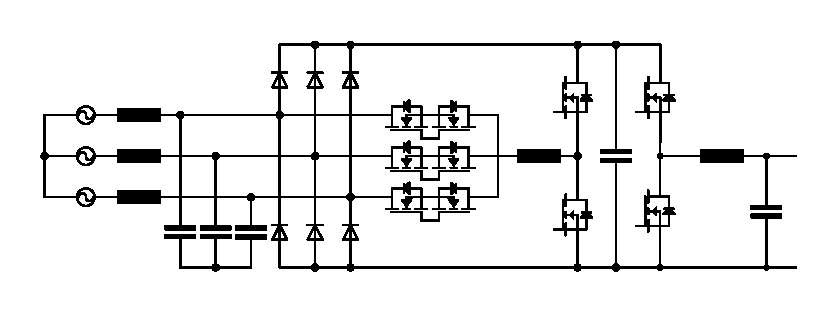
\includegraphics[width=0.9\linewidth]{content/Grafiken/IAF}
	\caption[\gls{IAF} Gleichrichter Topologie]{\gls{IAF} Gleichrichter Topologie}
	\label{fig:iaf}
\end{figure}


\section{1/3 PWM PFC Rectifier}
\label{sec:GrundlagenB6}
Bei dieser Topologie handelt es sich um eine verbreitete B6-Topologie, die aus drei Halbbrücken besteht die jeweils an einer Phase angeschlossen sind. Durch ein adaptives Modulationsverfahren, unter Verwendung von Induktivitäten auf der Netzseite, wird eine Reduzierung der Schaltverluste und \gls{SDL} ermöglicht. Das Verfahren wurde ausführlich von Menzi, Bortis und Kolar beschrieben \cite{13PWMPFC}. Zur Regelung der Ausgangsspannung wird ein entkoppelter Tiefsetzsteller eingesetzt.\\



\begin{figure}
	\centering
	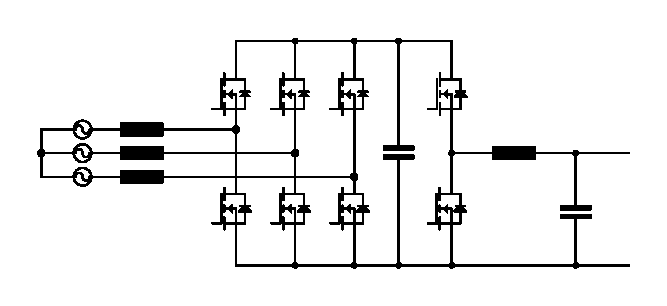
\includegraphics[width=0.9\linewidth]{content/Grafiken/B6_Buck}
	\caption[1/3 PWM PFC Buck]{1/3 PWM PFC Buck}
	\label{fig:b6buck}
\end{figure}

Das besondere an der Regelung ist es, dass die Phase die aktuell keinen Strom führt, da Sie die niedrigste Spannung hat, durch \gls{PWM} Ansteuerung der zugehörigen Halbbrücke einen passenden Stromfluss erreicht. Die beiden anderen Halbbrücken werden jeweils wie ein Diodengleichrichter geschaltet. Dieses verfahren ist vom Prinzip her das gleiche, wie beim \gls{IAF} und kann daher zum Verständnis gemeinsam betrachtet werden, siehe Abb. \ref{fig:b6iafsectors}.
Im hervorgehobenen Abschnitt ist Phase b am niedrigsten und es ist zu sehen, in Bereich (f), dass nur eine Halbbrücke per \gls{PWM} angesteuert wird. In Bereich (e) wird der Tastgrad \gls{D} dargestellt, wobei der Wert 1 die dauerhafte Verbindung zum positiven und -1 die zum negativen Potential des Zwischenkreis \gls{Upn} darstellt \cite{13PWMPFC}.\\ 

\begin{figure}
	\centering
	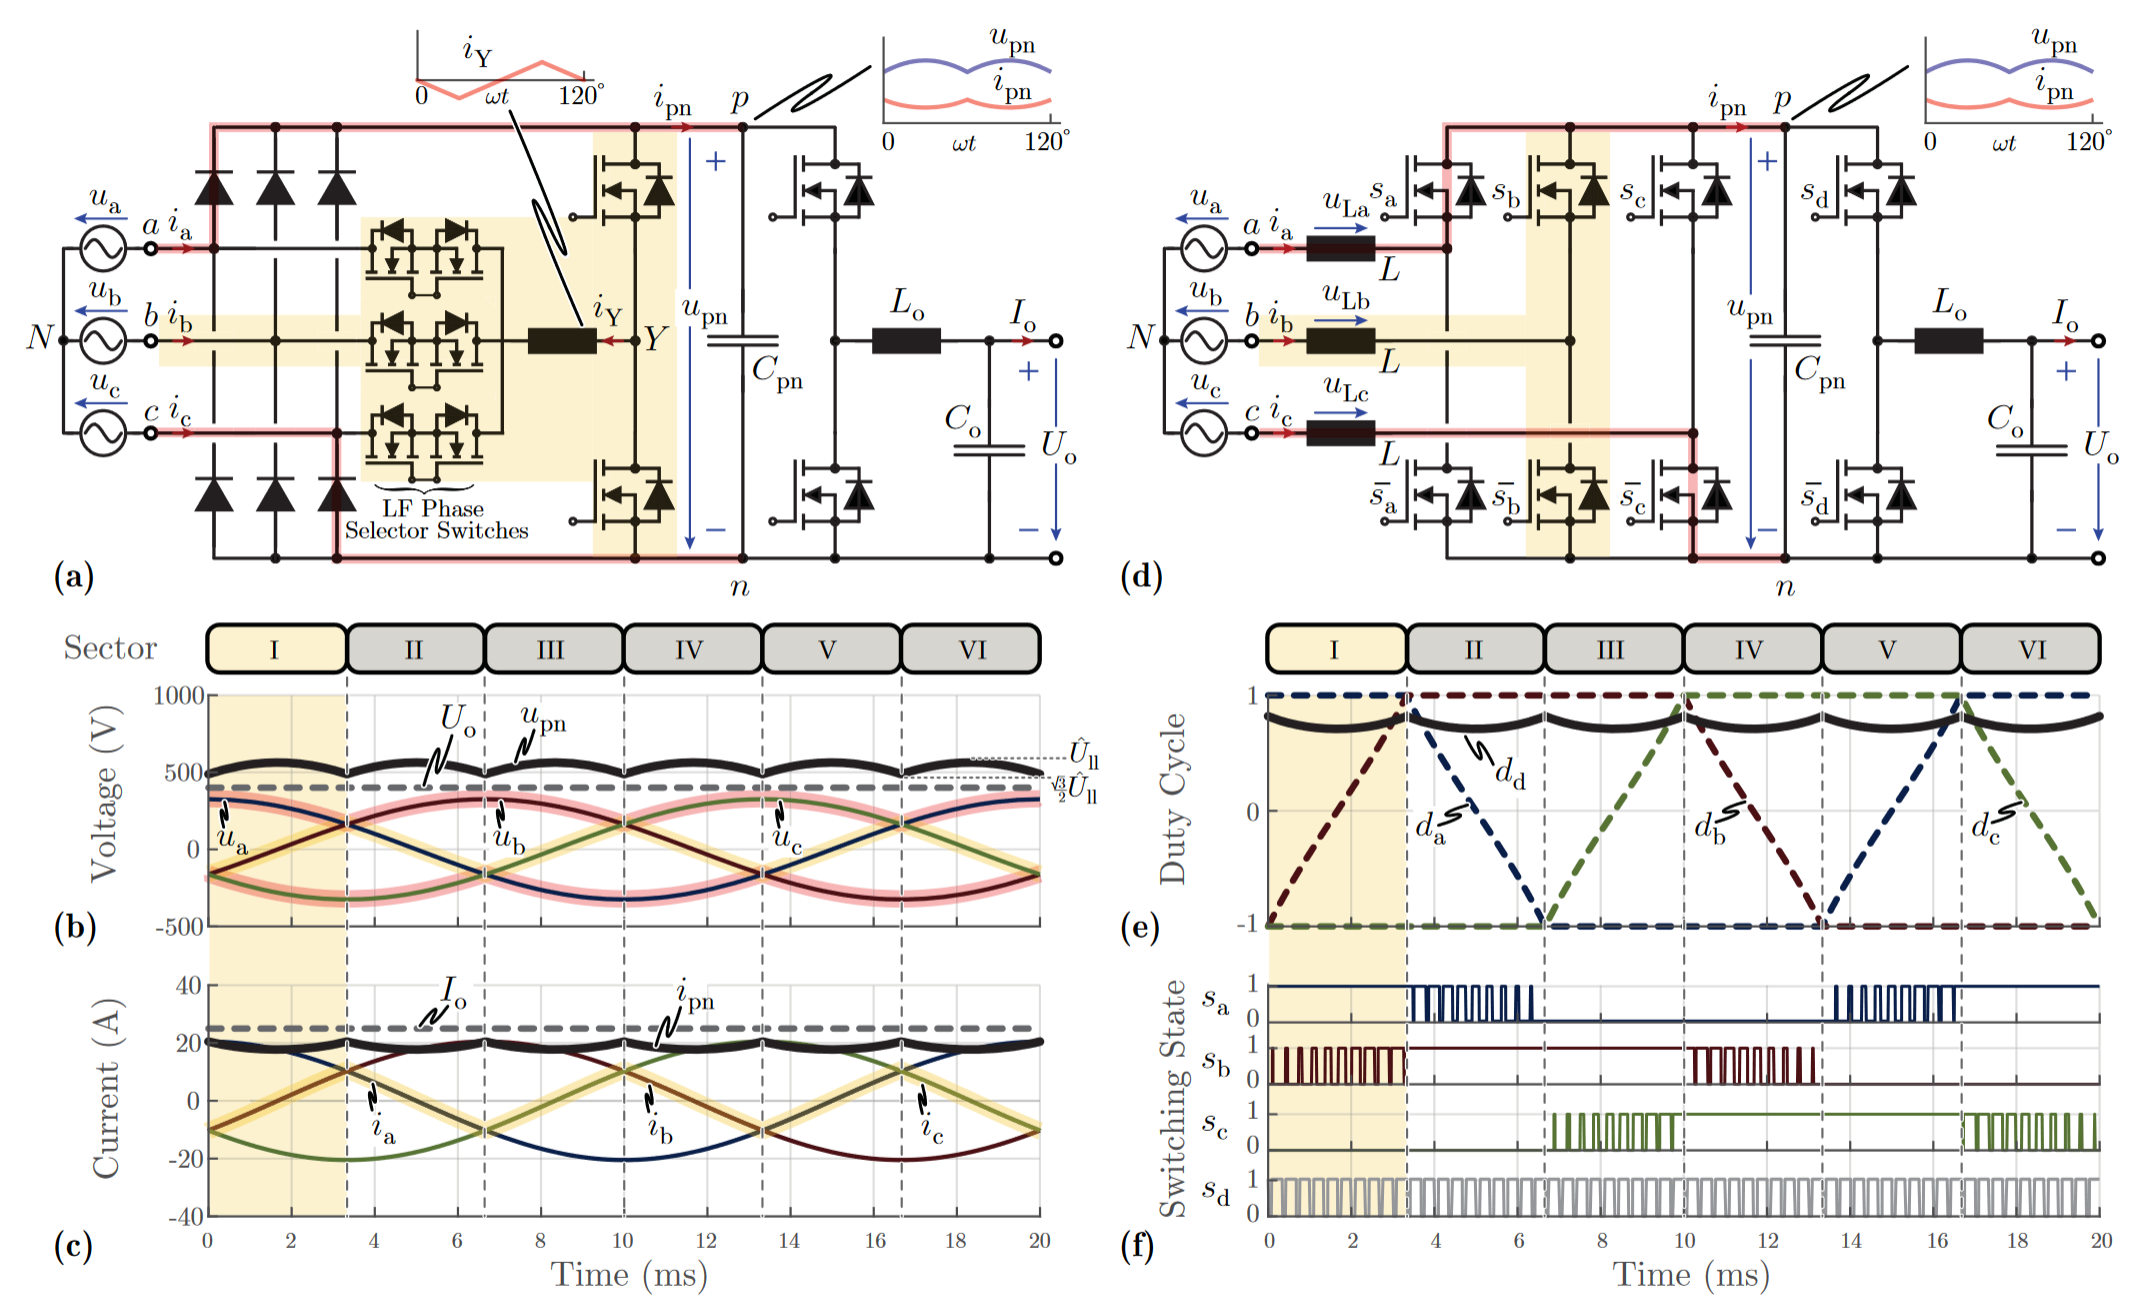
\includegraphics[width=0.9\linewidth]{content/Grafiken/B6+IAF_Sectors.png}
	\caption[Sektorenaufteilung und Schaltverhalten von IAF und B6 1/3 \cite{13PWMPFC}]{}
	\label{fig:b6iafsectors}
\end{figure}

\section{Leistungshalbleiter}
Halbleiter sind prinzipiell alle Komponenten mit mindestens einem PN-Übergang, wenn diese größere Leistungen Schalten können, werden sie als Leistungshalbleiter bezeichnet. Dazu sind für die verwendete Topologie, neben der klassischen Diode, \gls{MOSFET}  relevant. Diese lösen in der Leistungselektronik aktuell den verbreiteteren IGBT oftmals ab aufgrund der günstiger gewordenen Silicium Carbide Variante \cite{SiCTrend}. Die Vorteile dieser neuen Technologie liegen in der Ermöglichung höherer Schaltfrequenzen, dies wiederum ermöglicht die Reduzierung der Energie welche in den Induktiven Komponenten gespeichert werden muss und spart somit Kosten.\\
Um die am besten geeigneten Halbleiter auszuwählen werden u.a. Simulationen der Schaltung verwendet, diese benötigen eine Nachbildung der Halbleiter. Um die Modelle der Leistungshalbleiter zu erstellen und ggf. vorhandene zu validieren, können Messungen mittels \gls{DPT} durchgeführt werden. Ein Beispiel der in \gls{PLECS} dargestellten Ausschaltverluste für einen Halbleiter können in Abb. \ref{fig:plecsff2thermalmodel} gefunden werden. Es ist zu sehen, dass die Punkte nur für den Betriebspunkt von 600 Volt zur Verfügung stehen, für andere Betriebsbereiche muss das Verhalten approximiert werden. Außerdem wird der \gls{RGV} nur für einen Begrenzten Bereich dargestellt und die \gls{VGSS} nur auf einen Wert beschränkt. Dies kann für die spätere Anwendung zu deutlichen Abweichungen führen.
\begin{figure}
	\centering
	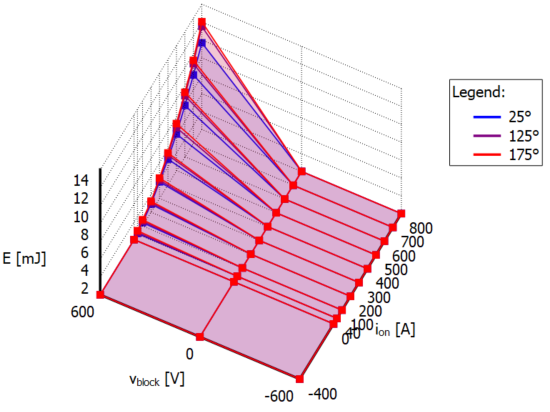
\includegraphics[width=0.7\linewidth]{content/Grafiken/PLECS_FF2ThermalModel}
	\caption[Darstellung der Ausschaltverluste \cite{IFAGFF2}]{Darstellung der Ausschaltverluste \cite{IFAGFF2}}
	\label{fig:plecsff2thermalmodel}
\end{figure}

\section{Induktive Komponenten}
Als Induktive Komponenten werden in der Regel Spulen und Transformatoren betrachtet, diese dienen dazu Energie zu Speichern und zu Übertragen. Transformatoren bieten zusätzlich die Möglichkeit der galvanischen Entkopplung von Stromkreisen.\\ 
Zur Auslegung von Induktivitäten wird das Delta des Stroms in der Spule benötigt, der sogenannte Stromrippel. Dieser Strom wird meist auf 30 Prozent des Effektivstroms ausgelegt. Der Rippelstrom für Drehstromsysteme kann über Formel \ref{eq:DeltaI} bestimmt werden. Dabei ist die \gls{S} und \gls{Ull} die Spannung zwischen den Außenleitern.\\
\begin{equation}
	\label{eq:DeltaI}
	 \Delta I = 0,3 \cdot \dfrac{\sqrt{2} \cdot S}{2 \cdot \sqrt{3} \cdot U_{LL}}
\end{equation}
Außerdem kann über die gespeicherte Energie in der Drossel eine Aussage darüber getroffen werden, wie groß und damit indirekt wie viel kosten und Platzbedarf diese benötigt.

FORMELN MIT QUELLENNN!!!!!!



\section{Simulationssoftware}
Zur Bewertung und Betrachtung der Umsetzbarkeit, der Topologien ist es nötig diese in einer Umfassenden Simulation zu betrachten. Dies ermöglicht es die Funktionalität und den Einfluss der Parameter im direkten Zusammenspiel zu untersuchen. Insbesondere das Verhalten für Systemdienstleistungen, wie Phasenverschiebung und die dadurch beeinflusste Verteilung der Verlustleistungen sollen als Entscheidungsgrundlage dienen. 

	\subsection{PLECS}
	Die Software \gls{PLECS} aus dem Haus PLEXIM wird als Integration in MATLAB mit Simulink verwendet.  Diese ermöglicht die Modellierung von Schaltungen mit der Betrachtung des Thermischen Verhaltens durch elektrische Modelle der Verlustleistung. Dazu wird die Energie im Schaltvorgang sowie im durchgeschalteten Zustand in der Schaltung berücksichtigt. Dies ermöglicht es die Verlustleistung innerhalb der Halbleiter zur betrachten und damit den Aufwand für die Kühlung und eine Abschätzung der Schaltungseffizienz. Ein Beispiel der Funktionen kann in Abb. \ref{fig:plecsbuck} gesehen werden, die thermische Kette muss anhand von Datenblättern oder ähnlichem der Kühlkörper bekannt sein. Für die Halbleiter werden thermische Modelle benötigt, die ebenfalls aus Datenblättern erstellt oder vom Hersteller bereitgestellt werden können. Jedoch gibt es nicht für alle Halbleiter ausreichend Informationen und die reale Verlustleistung hängt von vielen Parametern ab. Daher wird es oftmals benötigt eigene Messungen durchzuführen, um die spätere Anwendung bestmöglich simulieren zu können.   \\
	
	\begin{figure}
		\centering
		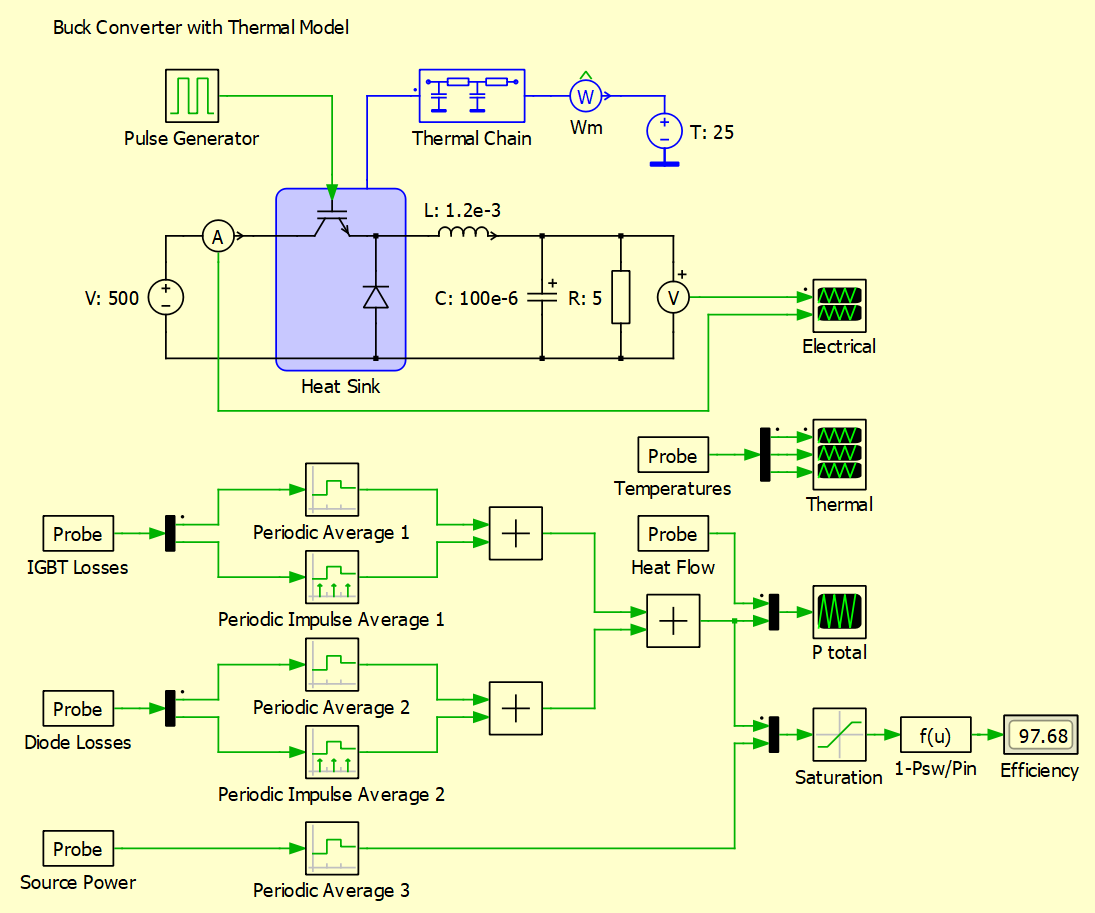
\includegraphics[width=0.9\linewidth]{content/Grafiken/PLECS_Buck}
		\caption[Tiefsetzsteller mit Effizienzbestimmung]{Tiefsetzsteller mit Effizienzbestimmung}
		\label{fig:plecsbuck}
	\end{figure}
	